\section{Terminology}\label{terminology}

Our research aims to describe the current state of software testing literature,
including its flaws. Since we critique the lack of clarity, consistency, and
robustness in the literature, we need to hold ourselves to a high standard in
these areas when defining and using terms. For example, since we focus
on how the literature describes ``test approaches'', we first define this term
(\Cref{approach-def}). Likewise, before we can constructively describe
the flaws in the literature, we need to define what we mean by ``flaw''
(\Cref{flaw-def}). To further prevent bias, we only use classifications and
relations already implicitly present in the literature instead of
inventing our own; for example, test approaches can have categories
(\Cref{cats-def}), synonyms (\Cref{syn-rels}), and parent-child relations
(\Cref{par-chd-rels}). We also observe flaws having both manifestations
(\Cref{mnfst-def}) and domains (\Cref{dmn-def})\thesisissueref{155} and use
these terms to refer to these implicit concepts in the literature. All of these
classifications and relations follow logically from the literature and as such
are technically ``results'' of our research, but we define them here for
clarity since we use them throughout this \docType{}.

Since the literature is flawed, we need to be careful with what information we
take at face value. We do this by tracking the nuance, or ``explicitness''%
\thesisissueref{176}, of information (\Cref{explicitness}) found in sources and
the ``credibility'' of these sources themselves (\Cref{cred}). We then use this
heuristic of credibility to group our identified sources into ``tiers''
(\Cref{source-tiers}). Defining these terms helps reduce the effect of our
preconceptions on our analysis (or at least makes it more obvious to future
researchers), as there may be other equally valid ways to analyze the
literature and its flaws. To be clear: we do \emph{not} prescribe what
terminology software testers \emph{should} use, we simply observe the
terminology that the literature uses and try to use it as consistently and
logically as possible.

\ifnotpaper\newpage\fi
\subsection{Test Approaches}\label{approach-def}

Software testing is defined as the ``process of operating a system or component
under specified conditions, observing or recording the results, and making an
evaluation of some aspect of the system or component'' \citep{ISO_IEC2014}%
%                     or ``the process of executing a program 
\todo{OG IEEE, 1990}\ifnotpaper, usually ``with the intent of finding errors''
(\citealp{Myers1976}, as cited in \citealp[p.~438]{PetersAndPedrycz2000}%
\footnote{See \flawref{myers-citation}.})\fi.
For each test, the main steps are to:
\begin{enumerate}
    \item identify the goal(s) of the test,
    \item \phantomsection{}\label{step:decide-app} decide on an approach,
    \item develop the tests,
    \item determine the expected results,
    \item \phantomsection{}\label{step:run-tests} run the tests, and
    \item \phantomsection{}\label{step:cmp-results} compare the expected results to
          the actual results \ifnotpaper \citetext{p.~443}\else
              \cite[p.~443]{PetersAndPedrycz2000}\fi.
          %   Only step 6 is similar in Firesmith2015; exclude for simplicity
          %   \ifnotpaper \citep[p.~443; similar in][p.~11]{Firesmith2015}
          %   \else \citetext{p.~443} (similar in \cite[p.~11]{Firesmith2015}) \fi
\end{enumerate}
The end goal is to evaluate ``some aspect of the system or component'' based on
the results of step~\ref{step:cmp-results} \ifnotpaper (\citealp[p.~10]{IEEE2022};
    \citeyear[p.~6]{IEEE2021c}; \citealp{ISO_IEC2014}\todo{OG IEEE, 1990})\else
    \cite[p.~10]{IEEE2022}, \cite[p.~6]{IEEE2021c}, \cite{ISO_IEC2014}\fi.
When this evaluation reveals errors, ``the faults causing them are what can and
must be removed'' \citep[p.~5\=/3]{SWEBOK2024}.

Of course, the approach chosen in step~\ref{step:decide-app} influences what
kinds of test cases should be developed and executed in later steps, so it is
important that test approaches are defined correctly, consistently, and
unambiguously.
% How the literature describes these approaches is the focus of our research.
A ``test approach'' is a ``high-level test implementation
choice'' \citep[p.~10]{IEEE2022} used to ``pick the particular test case
values'' \citeyearpar[p.~465]{IEEE2017} used in step~\ref{step:run-tests}. The only
approach that can ``fully'' test a system (exhaustive testing) is infeasible in
most non-trivial situations \ifnotpaper (\citeyear[p.~4]{IEEE2022};
    \citealp[p.~5\=/5]{SWEBOK2024}; \citealp[pp.~439, 461]{PetersAndPedrycz2000};
    \citealp[p.~421]{vanVliet2000})\else
    \cite[pp.~439, 461]{PetersAndPedrycz2000}, \cite[p.~421]{vanVliet2000},
    \cite[p.~5\=/5]{SWEBOK2024}, \cite[p.~4]{IEEE2022}\fi, so multiple
approaches are needed \ifnotpaper \citep[p.~18]{IEEE2022} \else
    \citetext{p.~18} \fi to ``suitably cover any system'' \citetext{p.~33}.
This is why this process should be repeated and there are so many test
approaches described in the literature.
% We record \approachCount{} test approaches mentioned in
% the literature in \ourApproachGlossary{}, along with their properties and
% relations. This includes any categories (\Cref{cats-def}), synonyms
% (\Cref{syn-rels}), and parent-child relations (\Cref{par-chd-rels}) described
% by the literature.

% that includes ``test level, test type, test technique, test practice and
% \dots{} static testing'' \citep[p.~10]{IEEE2022} and is used to  & black or white box, minimum and maximum
% boundary value testing \citep[p.~465]{IEEE2017}                                                  \\

\subsubsection{Approach Categories}\label{cats-def}

Since there are so many test approaches, it is helpful to categorize them.
The literature provides many ways to do so, but we use the one given by
\ifnotpaper\else \citeauthor{IEEE2022} \fi \citet{IEEE2022} because of its wide usage.
This schema divides test approaches into levels, types, techniques, and practices
\citeyearpar[Fig.~2; see \Cref{tab:ieeeCats}]{IEEE2022}. These categories seem
to be pervasive throughout the literature, particularly ``level'' and ``type''.
\phantomsection{}\label{nonIEEE-sources}%
For example, six non-IEEE sources also give unit testing, integration testing,
system testing, and acceptance testing as examples of test levels \ifnotpaper
    (\citealp[pp.~5\=/6 to 5\=/7]{SWEBOK2024}; \citealpISTQB{};
    \citealp[pp.~807\==808]{Perry2006}; \citealp[pp.~443\==445]{PetersAndPedrycz2000};
    \citealp[p.~218]{KuļešovsEtAl2013}\todo{OG Black, 2009};
    \citealp[pp.~9, 13]{Gerrard2000a})\else
    \cite[pp.~443\==445]{PetersAndPedrycz2000},
    \cite[pp.~5\=/6 to 5\=/7]{SWEBOK2024}, \cite{ISTQB},
    \cite[pp.~807\==808]{Perry2006}, \cite[pp.~9, 13]{Gerrard2000a},
    \cite[p.~218]{KuļešovsEtAl2013}\fi.\phantomsection{}\label{orth-approach}
These categories seem to be orthogonal based on their definitions and usage.
For example, ``a test type can be performed at a single test level or across
several test levels'' \ifnotpaper (\citealp[p.~15]{IEEE2022};
    \citeyear[p.~8]{IEEE2021a}; \citeyear[p.~7]{IEEE2021c})\else
    \cite[p.~15]{IEEE2022}, \cite[p.~7]{IEEE2021c}, \cite[p.~8]{IEEE2021a}\fi,
and test practices can be ``defined \dots{} for a specific level or type of
testing'' \citeyearpar[p.~9]{IEEE2021b}.
% , and ``Keyword-Driven Testing can be applied at all testing levels
% \dots{} and for various types of testing'' \citeyearpar[p.~4]{IEEE2016}.
% Therefore, we assume these categories to be orthogonal throughout this
% \docType{} (e.g., when identifying flaws).
We may assess this assumption more rigorously in the future, but for now, it
implies that one can derive a specific test approach by combining multiple
test approaches from different categories\ifnotpaper
    %. For example, usability test
    % script(ing) \citepISTQB{} is a combination of usability testing, a test type
    % \ifnotpaper (\citealp[pp.~22, 26--27]{IEEE2022};
    %     \citeyear[pp.~7, 40, Tab.~A.1]{IEEE2021c}; implied by its quality;
    %     \citealp[p.~53]{Firesmith2015})\else \cite[pp.~22, 26--27]{IEEE2022},
    %     \cite[pp.~7, 40, Tab.~A.1]{IEEE2021c}\fi, and scripted testing, a test
    % practice \citep[pp.~20, 22\ifnotpaper; implied by p.~33\fi]{IEEE2022}
    ; see \Cref{orth-test} for more detailed discussion\fi.
% Because of their widespread use and their usefulness in dividing the domain of
% software testing into more manageable subsets, we use these categories
% throughout this \docType{}.
We loosely describe these categories based on what they specify
as follows\thesisissueref{21}:
\begin{itemize}
    \item \textbf{Level}: What code is tested
    \item \textbf{Practice}: How the test is structured and executed
    \item \textbf{Technique}: How inputs and/or outputs are derived
    \item \textbf{Type}: Which software quality is evaluated
\end{itemize}

% For example, static assertion checking (mentioned by \ifnotpaper
%     \citealp[p.~345]{LahiriEtAl2013}; \citealp[p.~343]{ChalinEtAl2006}\else
%     \citealp[p.~343]{ChalinEtAl2006}, \citealp[p.~345]{LahiriEtAl2013}\fi) is a
% subapproach of assertion checking, which can also be performed dynamically.
% This parent-child relation (defined in \Cref{par-chd-rels}) means that static
% assertion checking may inherit assertion checking's inferred category of
% ``practice''. Based on observations such as this, we categorize testing
% approaches, \emph{including} static ones, based on the remaining categories
% from \citet{IEEE2022}.
% \ifnotpaper However, since there are many ways to categorize test approaches
%     (see \Cref{tab:otherCats,tab:otherCategorizations}), considering static
%     testing as an orthogonal distinction could make sense in specific contexts
%     (see \Cref{static-test}).

% % Removed for brevity; #202
% For example, boundary value analysis is a test technique since its inputs are
% ``the boundaries of equivalence partitions'' \ifnotpaper
%     (\citealp[p.~2]{IEEE2022}; \citeyear[p.~1]{IEEE2021c}; similar on p.~12;
%     \citealpISTQB{})%
% \else
%     \cite[p.~2]{IEEE2022}, \cite[p.~1]{IEEE2021c}%
% \fi. Similarly, acceptance testing is a test level since its goal is to
% ``enable a user, customer, or other authorized entity to determine whether to
% accept a system or component'' \ifnotpaper (\citealp[p.~5]{IEEE2017}; similar
%     in \citeyear[p.~6]{IEEE2021c}; \citealp[p.~344]{SakamotoEtAl2013})\else
%     \cite[p.~5]{IEEE2017}\fi, which requires the system or component to be
% developed and ready for testing.

% Based on how we observe test approaches being categorized in the literature, 
% We also make the following changes to the schema from \citet[Fig.~2]{IEEE2022}:

While \citet{IEEE2022}'s schema includes ``static testing'' as a test approach
category, we omit it from our scope as it seems non-orthogonal to the others
and thus less helpful for grouping test approaches. \ifnotpaper Other
    categorization schemas (see \Cref{alt-cats}) may consider static testing
    orthogonal, and some may consider it out-of-scope entirely (see
    \Cref{static-test})! \fi We also introduce a ``supplemental'' category of
``artifact''\thesisissueref{44,119,39} since some terms can refer to both the
application of a test approach \emph{and} the resulting document(s).
\ifnotpaper
    These two ideas are sometimes explicitly distinguished, such as
    ``conformity evaluation'' and ``conformity evaluation report''
    \citep{ISO_IEC2014}, but often are not.
    % Additionally, \citet[p.~3]{SouzaEtAl2017} give ``test procedures'', which
    % may be considered equivalent to ``test approaches''
    % (see \Cref{tab:otherCats}), as examples of testing artifacts.
\fi
% The role of testing artifacts is not specified in \citep{BarbosaEtAl2006};
% requirements, drivers, and source code are all treated the same
% with no distinction \citep[p.~3]{BarbosaEtAl2006}.
Therefore, we do \emph{not} consider approaches categorized as an artifact
\emph{and} another category as flaws\thesisissueref{119} in \Cref{multiCats}.
Finally, we also record the test category of ``process'' for completeness,
although this seems to be a higher level classification and these approaches
will likely be excluded during later analysis\thesisissueref{52}.

\ifnotpaper
    % \afterpage{
    \begin{landscape}
        \begin{table*}[p]
            % Moved earlier to display nicely in paper
            \ieeeCatsTable{}
        \end{table*}
    \end{landscape}
    % }
\fi

% \fi
% While we can categorize the vast majority of identified test approaches
% based on \citet{IEEE2022}'s categories, there are some outliers. For example,
% we categorize some test approaches as ``artifacts'',
% since some terms can refer to the application of a
% test approach \emph{as well as} the resulting document(s). Therefore,
% \ifnotpaper
%     Additionally, we identify ``test metrics''\thesisissueref{21,22} that
%     describe methods for \emph{evaluating} testing as opposed to methods for
%     \emph{performing} it and are therefore out-of-scope. Instead,
%     we capture the related test approaches that seek to maximize these
%     metrics as subsets of coverage-driven testing (see \Cref{cov-test}) and
%     experience-based testing \citep[p.~34]{IEEE2022}.
% \fi

\subsubsection{Synonym Relations}\label{syn-rels}

The same approach often has many names. For example,
``specification-based testing'' is also called
% \todo{more in Umar2000}:
% \begin{enumerate}
%     \item 
``black-box testing''
\def\noHyphenFn{\footnote{\refHelper \citet{Firesmith2015} excludes the hyphen,
        calling it ``black box testing''.}}
\ifnotpaper
    (\citealp[p.~9]{IEEE2022}; \citeyear[p.~8]{IEEE2021c};
    \citeyear[p.~431]{IEEE2017}; \citealp[p.~5\=/10]{SWEBOK2024};
    \citealpISTQB{}; \citealp[pp.~46\==47\noHyphenFn]{Firesmith2015};
    \citealp[p.~344]{SakamotoEtAl2013}; \citealp[p.~399]{vanVliet2000})\else
    \cite[pp.~46\==47\noHyphenFn]{Firesmith2015}, \cite[p.~399]{vanVliet2000},
    \cite[p.~5\=/10]{SWEBOK2024}, \cite[p.~431]{IEEE2017},
    \cite[p.~9]{IEEE2022}, \cite{ISTQB}, \cite[p.~8]{IEEE2021c},
    \cite[p.~344]{SakamotoEtAl2013}\fi.
%     \item ``closed-box testing''
%           \ifnotpaper
%               (\citealp[p.~9]{IEEE2022}; \citeyear[p.~431]{IEEE2017})
%           \else
%               \cite[p.~431]{IEEE2017}, \cite[p.~9]{IEEE2022}
%           \fi
%     \item ``functional testing''\footnote{``Functional testing'' may not
%               \emph{actually} be a synonym for ``specification-based testing'';
%               see \flawref{spec-func-syn}.}
%           \ifnotpaper
%               (\citealp[p.~196]{IEEE2017}; \citealp[p.~44]{Kam2008};
%               \citealp[p.~399]{vanVliet2000}; implied by
%               \citealp[p.~129]{IEEE2021c}; \citeyear[p.~431]{IEEE2017})
%           \else
%               \cite[p.~399]{vanVliet2000}, \cite[p.~196]{IEEE2017},
%               \cite[p.~44]{Kam2008} (implied by \cite[p.~431]{IEEE2017},
%               \cite[p.~129]{IEEE2021c})
%           \fi
%     \item ``domain testing'' \citep[p.~5\=/10]{SWEBOK2024}
%     \item ``specification-oriented testing'' \citep[p.~440, Fig.~12.2]{PetersAndPedrycz2000}
%     \item ``input domain-based testing'' (implied by \citealp[pp.~4\=/7 to
%               4\=/8]{SWEBOK2014})
% \end{enumerate}
Throughout our work, we use the terms
``specification-based testing'' and ``structure-based testing'' to articulate
the source of the information for designing test cases, but a team or project
also using grey-box testing may prefer the terms ``black-box'' and ``white-box
testing'' for consistency.

\defRel{synonym}{S}{how synonyms are used in natural language}
$S$ is symmetric and transitive, and although pairs of
synonyms in natural language are implied to be distinct, a relation that is
symmetric and transitive is provably reflexive; this implies that all terms are
trivially synonyms of themselves. Since $S$ is symmetric, transitive,
\emph{and} reflexive, it is an equivalence relation, reflecting the role of
synonyms in natural language where they can be used interchangeably. While
synonyms may emphasize different aspects or express mild variations, their core
meaning is nevertheless the same.

%%  Removed for brevity, but may be used elsewhere; #183

% As an example of synonyms in natural language, ``windy'' is a synonym of
% ``gusty'' \citep{WindySyns}; since this is a symmetric relation, the inverse is
% also true \citeyearpar{GustySyns}. ``Windy'' is also a synonym of ``blustery''
% \citeyearpar{WindySyns}, so since this relation is transitive and ``gusty'' is
% a synonym of ``windy'', ``gusty'' is also a synonym of ``blustery''
% \citeyearpar{GustySyns}. Although these terms are distinct
% \citeyearpar{GustySyns,WindySyns} and have nuance---``gust'' is defined as ``a
% sudden brief rush of wind'' \citeyearpar{GustDef}---they still reflect the
% same core concept and could be considered synonyms of themselves.

% Synonym relations are often given explicitly in the literature. For example,
% \citet[p.~9]{IEEE2022} \multiAuthHelper{list} ``black-box testing'' and
% ``closed box testing'' beneath the glossary entry for ``specification-based
% testing'', meaning they are synonyms. ``Black-box testing'' is likewise given
% under ``functional testing'' in \citeyearpar[p.~196]{IEEE2017}, so it is
% also a synonym for ``specification-based testing'' through transitivity.
% However, these relations can also be implicit (see \Cref{explicitness});
% ``functional testing'' is listed in a \emph{cf.} footnote to the glossary entry
% for ``specification-based testing'' \citeyearpar[p.~431]{IEEE2017}, which
% supports the previous claim but would not necessarily indicate a synonym
% relation on its own.

% Similarly, \citet[p.~5\=/10]{SWEBOK2024} says ``\emph{specification-based
%     techniques} \dots{} [are] sometimes also called domain
% testing techniques'' in the \acs{swebok} V4, from which the synonym of
% ``domain testing'' follows logically. However, its predecessor V3 only
% \emph{implies} the more specific ``input domain-based testing'' as a synonym.
% The section on test techniques says ``the classification of testing techniques
% presented here is based on how tests are generated: from the software
% engineer's intuition and experience, the specifications, the code structure
% \dots'' \citep[p.~4\=/7]{SWEBOK2014}, and the first three subsections on the
% following page are ``Based on the Software Engineer's Intuition and
% Experience'', ``Input Domain-Based Techniques'', and ``Code-Based Techniques''
% \citetext{p.~4\=/8}. The order of the introductory list lines up with these
% sections, implying that ``input domain-based techniques'' are ``generated[]
% from \dots{} the specifications'' (i.e., that input domain-based testing is the
% same as specification-based testing). Furthermore, the examples of input
% domain-based techniques given---equivalence partitioning, pairwise testing,
% boundary-value analysis, and random testing---are all given as children%
% \footnote{
%     Pairwise testing is given as a child of combinatorial testing, which is
%     itself a child of specification-based testing, by \ifnotpaper
%         \citep[Fig.~2]{IEEE2021c} and \citep[pp.~5\=/11 to 5\=/12]{SWEBOK2024}%
%     \else
%         \cite[pp.~5\=/11 to 5\=/12]{SWEBOK2024} and \cite[Fig.~2]{IEEE2021c}%
%     \fi, making it a ``grandchild'' of specification-based testing according to
%     these sources.
% } of specification-based testing \ifnotpaper
%     (\citealp{IEEE2022}; \citeyear[Fig.~2]{IEEE2021c}; \citealpISTQB{})\else
%     \cite{IEEE2022,ISTQB}, \cite[Fig.~2]{IEEE2021c}\fi; even V4 agrees with
% this \citep[pp.~5\=/11 to 5\=/12]{SWEBOK2024}!

\subsubsection{Parent-Child Relations}\label{par-chd-rels}
Many test approaches are multi-faceted and can be ``specialized'' into others;
for example, load testing and stress testing are some subtypes of
performance-related testing (described in more detail in \Cref{perf-test-rec}).
We refer to these ``specializations'' as ``children'' or ``subapproaches'' of
their multi-faceted ``parent(s)''. This nomenclature also extends to approach
categories (such as ``subtype''; see \Cref{cats-def,tab:ieeeCats}) and software
qualities (``subquality''\ifnotpaper; see \Cref{qual-supp-procedure}\fi).

\defRel{parent-child}{P}{directed relations between approach pairs} This
relation should be irreflexive, asymmetric, and transitive, making it a strict
partial order. A consequence of this is that there should be no directed
cycles, although since a given child approach $c$ may have more than one
parent approach $p$, undirected cycles may exist\qtodo{Is this precise enough?}.

Parent-child relations often manifest when a ``well-understood'' test approach
$p$ is decomposed into smaller, independently performable approaches
$c_1, \dots, c_n$, each with its own focus or nuance. This is frequently the
case for hierarchies of approaches given in the literature \ifnotpaper
    (\citealp[Fig.~2]{IEEE2022}; \citeyear[Fig.~2]{IEEE2021c};
    \citealp{Firesmith2015})\else \cite{Firesmith2015},
    \cite[Fig.~2]{IEEE2022}, \cite[Fig.~2]{IEEE2021c}\fi.
%; see the graph of specification-based test approaches in \Cref{fig:specBasedGraph}
Another way for these relations to occur is when
% $c$'s adequacy criteria is already satisfied by $p$. In other words,
the completion of $p$ indicates that ``sufficient testing has been done'' in
regards to $c$ \citep[p.~402]{vanVliet2000}. While this only ``compares the
thoroughness of test techniques, not their ability to detect faults''
\citetext{p.~434}, it is sufficient to justify a parent-child relation
between the two approaches. These relations may also be represented as
hierarchies \ifnotpaper (\citealp[Fig.~F.1]{IEEE2021c};
    \citealp[Fig.~13.17]{vanVliet2000})\else
    \citetext{Fig.~13.17}, \cite[Fig.~F.1]{IEEE2021c}\fi.
%; see the graph of data flow test approaches in \Cref{fig:subsumesGraph}

% \parChdGraphs{}

% Based on what we observe in the literature,
% $P(c, p) = c \subset p \textrm{ or } c \Leftarrow p$. In other words,
% one of the following must be true:
% % There are many reasons two approaches may have a parent-child relation, such as:

% \begin{enumerate}
%     \item Everything described by $c$ is also described by $p$; $c \subset p$.
%           This is often the case when one ``well-understood'' subset of testing
%           can be decomposed into smaller, independently performable approaches,
%           each with its own focus or nuance. This is often the case for
%           hierarchies of approaches given in the literature \ifnotpaper
%               (\citealp[Fig.~2]{IEEE2022}; \citeyear[Fig.~2]{IEEE2021c};
%               \citealp{Firesmith2015})\else \cite{Firesmith2015},
%               \cite[Fig.~2]{IEEE2022}, \cite[Fig.~2]{IEEE2021c}\fi; we graph
%           the parent-child relations in the subdomain of specification-based
%           testing in \Cref{fig:specBasedGraph} as an example.
%     \item Completing $p$ implies that $c$ has also been completed; $c \Leftarrow p$.
%           This is really just a more specific case of the previous condition that
%           occurs when $c$'s adequacy criteria is already met by $p$. While
%           this relation only ``compares the thoroughness of test techniques, not
%           their ability to detect faults'' \citep[p.~434]{vanVliet2000}, it is
%           sufficient to constitute a parent-child relation. These may also be
%           represented as hierarchies \ifnotpaper (\citealp[Fig.~F.1]{IEEE2021c};
%               \citealp[Fig.~13.17]{vanVliet2000})\else
%               \citetext{Fig.~13.17}, \cite[Fig.~F.1]{IEEE2021c}\fi; we graph the
%           parent-child relations in the subdomain of data flow testing in
%           \Cref{fig:subsumesGraph} as an example.
% \end{enumerate}

% \begin{enumerate}
%     \item \textbf{One is a superset of the other.} In other words, for one
%           (parent) test approach to be performed in its entirety, the other
%           (child) approach will necessarily be performed as well. This is often
%           the case when one ``well-understood'' subset of testing can be
%           decomposed into smaller, independently performable approaches.
%           When all of these have been completed, we can logically conclude that
%           the parent approach has also been performed! In practice, this is
%           much harder to prove; although many hierarchies exist \ifnotpaper
%               (\citealp[Fig.~2]{IEEE2022}; \citeyear[Fig.~2]{IEEE2021c};
%               \citealp{Firesmith2015})\else \cite{Firesmith2015},
%               \cite[Fig.~2]{IEEE2022}, \cite[Fig.~2]{IEEE2021c}\fi, these are
%           likely incomplete. As an example, we graph the parent-child relations
%           from \ifnotpaper (\citealp[Fig.~2]{IEEE2022}; \citeyear[Fig.~2]{IEEE2021c})
%           \else \cite[Fig.~2]{IEEE2022}, \cite[Fig.~2]{IEEE2021c} \fi in the
%           subdomain of specification-based testing in \Cref{fig:specBasedGraph}
%           (along with relevant data from other sources).
%     \item \textbf{One is ``stronger than'' or ``subsumes'' the other.} When
%           comparing adequacy criteria that ``specif[y] requirements for
%           testing'' \citep[p.~402]{vanVliet2000}, ``criterion X is stronger
%           than criterion Y if, for all programs P and all test sets T,
%           X-adequacy implies Y-adequacy'' \citetext{p.~432}. While this
%           relation only ``compares the thoroughness of test techniques, not
%           their ability to detect faults'' \citetext{p.~434}, it is sufficient
%           to consider one a child of the other in a sense. We capture this
%           nuance by considering these parent-child relations implicit
%           (see \Cref{explicitness}). As an example, we graph the parent-child
%           relations from \ifnotpaper (\citealp[Fig.~F.1]{IEEE2021c};
%               \citealp[Fig.~13.17]{vanVliet2000}) \else
%               \citetext{Fig.~13.17}, \cite[Fig.~F.1]{IEEE2021c}
%           \fi in the subdomain of data flow testing can be found in
%           \Cref{fig:subsumesGraph} (along with relevant data from other sources).
%           \item \textbf{The parent approach is part of an orthogonal set.}
%                 When presented with a set of generic test approaches that are
%                 orthogonal to each other, it is often trivial to classify a given
%                 test approach as a child of just one them. For example,
%                 \citeauthor{IEEE2022} say that ``testing can take two forms: static
%                 and dynamic'' \citeyearpar[p.~17]{IEEE2022} and provide examples of
%                 subapproaches of static and dynamic testing \citetext{Fig.~1}.
%                 Likewise, \citeauthor{Gerrard2000a} says ``tests can be automated or
%                 manual'' \citeyearpar[p.~13]{Gerrard2000a} and gives subapproaches of
%                 automated and manual testing \ifnotpaper
%                     \citeyearpar[Tab.~2; ][Tab.~1]{Gerrard2000b}\else
%                     \citetext{Tab.~2}, \cite[Tab.~1]{Gerrard2000b}\fi. However, the
%                 orthogonality of these subsets does not mean they are mutually
%                 exclusive; in these same tables, \citeauthor{Gerrard2000a} labels
%                 usability testing as both static \emph{and} dynamic and 12 approaches
%                 as able to ``be done manually \emph{or} using a tool''
%                 \citeyearpar[p.~13\ifnotpaper, emphasis added\fi]{Gerrard2000a}.
% \end{enumerate}

\subsection{Flaws}\label{flaw-def}

% Before we can start tracking and discussing flaws, we need to be clear about
% what we mean by the term. 
Ideally, software testing literature would describe test approaches correctly,
completely, consistently, and modularly, but this is not the case in reality.
We use the term ``flaw'' to refer to any instance of the literature violating
these ideals, \emph{not} to instances of \emph{software} doing the same%
\footnote{When picking a word to describe these violations, we wanted to avoid
    words that are ``overloaded with too many meanings'' like
    ``error'' and ``fault'' \citep[p.~12\=/3; see \Cref{error-fault-failure}
        for more detailed discussion]{SWEBOK2024}. A small literature review
    revealed that established standards (see \Cref{stds}) use the term
    ``flaw'' to refer to requirements \citep[p.~38]{IEEE2022}, design
    \citetext{p.~43}, ``system security procedures \dots{} and internal
    controls'' % under the term ``vulnerability''
    \citep[p.~194]{IEEE2012}, but only once to refer to code itself
    \citetext{p.~92}. \refHelper
    \citet[p.~7\=/9]{SWEBOK2024} also uses the word ``flaw'' in a way that
    aligns with our goal of analyzing what is wrong with software
    engineering's testing literature.}\todo{Present tense in footnote?}.
% , as it implies that something is wrong with the literature and there is an
% opportunity to improve it
We classify flaws by both their ``manifestations'' (\emph{how} information is
wrong; see \Cref{mnfst-def}) and their ``domains'' (\emph{what} information is
wrong; see \Cref{dmn-def})\thesisissueref{155}. These are orthogonal
classifications, since each flaw \emph{manifests} in a particular
\emph{domain}, which we track by assigning each flaw one ``key'' for each
classification. We list these keys in \Cref{tab:flawMnfstDefs,tab:flawDmnDefs},
respectively, and use them to count and analyze the flaws we uncover
in \Cref{flaws}% ; for
% example, we present the number of flaws according to these two views in
% \Cref{tab:flawMnfsts,tab:flawDmns}, respectively
. We also introduce some terms
to be used when discussing flaws based on how many sources contribute to them
(\Cref{add-flaw-terms}).

\subsubsection{Flaw Manifestations}\label{mnfst-def}

Perhaps the most obvious example of something being ``wrong'' with the
literature is that a piece of information it presents is incorrect---``wrong''
in the literal sense. However, if our standards for correctness require
clarity, consistency, and robustness, then there are many ways for a flaw to
manifest. This is one view we take when observing, recording, and analyzing
flaws: \emph{how}\thesisissueref{155} information is ``wrong''. We observe the
``manifestations'' described in \Cref{tab:flawMnfstDefs} throughout the
literature, and give each a unique key for later analysis and discussion. We
list them in descending order of severity, although this is partially
subjective. While some may disagree with our ranking, it is clear that
information being incorrect is worse than it being repeated. Our ordering has
the benefit of serving as a ``flowchart'' for classifying flaws. For example,
if a piece of information is not intrinsically incorrect, then there are five
remaining manifestation types for the flaw. Note that some flaws involve
information from multiple sources (contradictions and overlaps in particular).
We do not categorize these flaws as ``mistakes'' if finding the ground truth
requires analysis that has not been performed yet.

\begin{table}[tb]
    \centering
    \begin{talltblr}[
        note{a} = {We use \texttt{WRONG} here to avoid clashing with \texttt{MISS}.},
        note{b} = {We use \texttt{MISS} here to be more meaningful in isolation,
                as it implies the synonym of ``missing''; \texttt{OMISS} is
                less intuitive and \texttt{OMIT} would be inconsistent with the
                keys being adjective-based.},
        caption = {Observed flaw manifestations.},
        label = {tab:flawMnfstDefs}
        ]{
        colspec={|Q[c,m]X[l,m]Q[c,m]|},
        column{3} = {font=\ttfamily}, row{1} = {font=\normalfont},
        width = \columnwidth, rowhead = 1
        }
        \hline
        \thead{Manifestation} & \thead{Description}                                   & \thead{Key}       \\
        \hline
        \wrong*{}             & Information is incorrect                              & WRONG\TblrNote{a} \\
        \miss*{}              & Information that should be included is not            & MISS\TblrNote{b}  \\
        \contra*{}            & Information from multiple places conflicts            & CONTRA            \\
        \ambi*{}              & Information is unclear                                & AMBI              \\
        \over*{}              & Information is nonatomic or used in multiple contexts & OVER              \\
        \redun*{}             & Information is redundant                              & REDUN             \\
        \hline
    \end{talltblr}
\end{table}

\subsubsection{Flaw Domains}\label{dmn-def}

Another way to categorize flaws is by \emph{what} information is wrong, which
we call the flaw's ``domain''. We describe those we observe in
\Cref{tab:flawDmnDefs}, and tracking these uncovers which knowledge domains
are less standardized (and should therefore be approached with more rigour)
than others. We explicitly define some of these domains in previous
sections and thus present them in that same order. These are the domains in
which we automatically detect flaws as described in \Cref{auto-flaw-analysis}
and present in \Cref{flawDmns}, so these are the only ones that are
hyperlinked. We automatically detect the following classes of flaws:

\begin{itemize}
    \item \multiCatIntro*{}
    \item \phantomsection{}\label{relevantSyns}
          Synonyms that violate transitivity (see \Cref{syn-rels}); if two
          distinct approaches share a synonym but are not synonyms themselves,
          at least one relation is incorrect or missing.
    \item Synonyms between independently defined approaches; if two separate
          approaches have their own definitions, nuances, etc.~but are also
          labelled as synonyms, this indicates that:
          \begin{enumerate}
              \item the terms are interchangeable and this relation is
                    trivially reflexive (see \Cref{syn-rels}),
              \item at least one of these terms is defined incorrectly, and/or
              \item this synonym relation is incorrect.
          \end{enumerate}
    \item \phantomsection{}\label{selfParDef}
          Parent-child relations that violate irreflexivity, or approaches that
          are parents of themselves.\todo{Mention detecting other cycles as
              flaws as Future Work}
    \item \phantomsection{}\label{parSynDef}
          \parSynFlaw*{}
\end{itemize}

\begin{table}[tb]
    \centering
    \begin{talltblr}[
        % note{a} = {We use \texttt{WRONG} here to avoid clashing with \texttt{MISS}.},
        caption = {Observed flaw domains.},
        label = {tab:flawDmnDefs}
        ]{
        colspec={|Q[c,m]X[l,m]Q[c,m]|},
        column{3} = {font=\ttfamily}, row{1} = {font=\normalfont},
        width = \columnwidth, rowhead = 1
        }
        \hline
        \thead{Subset of Flaws} & \thead{Knowledge Domain}                               & \thead{Key} \\
        \hline
        \cats{}                 & Approach categories, defined in \Cref{cats-def}        & CATS        \\
        \syns{}                 & Synonym relations, defined in \Cref{syn-rels}          & SYNS        \\
        \pars{}                 & Parent-child relations, defined in \Cref{par-chd-rels} & PARS        \\
        \defs{}                 & Definitions given to terms                             & DEFS        \\
        \terms{}                & Labels or names given to terms                         & TERMS       \\
        \cites{}                & Citation information                                   & CITES       \\
        \hline
    \end{talltblr}
\end{table}

Despite their nuance, the remaining domains are relatively straightforward, so
we define them briefly as follows instead of defining them more rigorously in
their own sections.\phantomsection{}\label{label-flaw-def}
\defLabelDistinct{}. Definition flaws are quite self-explanatory, but
% occur when a term's definition is incorrect, unclear, etc., which often
% occurs in glossaries or lists of terms from sources we investigate.
% On the other hand,
label flaws are harder to detect, despite occurring independently. Examples of
label flaws include terms that share the same acronym or contain typos or
redundant information. Sometimes, an author may use one term when they mean
another. One could argue that their ``internal'' definition of the term is the
cause of this mistake, but we consider this a label flaw where the wrong
label is used as we would change the \emph{label} to fix it.
\phantomsection{}\label{scope-flaw-def}% (see \flawref{assert-truth})
Additionally, some information is presented with an incorrect scope and
sometimes should not have been included at all!
\phantomsection{}\label{trace-flaw-def}% (see \flawref{see-ref-missing})
Finally, some traceability information is flawed, such as how one document
cites another or even what information is included \emph{within} a document.

\subsubsection{Additional Flaw Terminology}\label{add-flaw-terms}
Some flaws involve information from more than one source, but referring to this
as a ``flaw between two sources'' is awkward\thesisissueref{140}. We instead
refer to this kind of flaw as an ``inconsistency'' between the
sources. This clearly indicates that there is disagreement between
the sources, but also does not imply that either one is correct---the
inconsistency could be with some ground truth if \emph{neither} source is
correct\thesisissueref{140,151}!

\phantomsection{}\label{one-src-flaws}
Other flaws only involve one source, but \oneSrcDistinct{}
Self-contained flaws are those that manifest by comparing a document to an
assertion of ground truth. These may appear once in a document or consistently
throughout it. Sometimes, these do not require an explicit comparison to ground
truth; these often include omissions as the lack of information is
contained within a single source and does not need to be cross-checked against
an assertion of ground truth. On the other hand, internal flaws arise when a
document disagrees with itself by containing two conflicting pieces of
information; this includes many contradictions and overlaps. Internal flaws can
even occur on the same page, such as when a source gives the same acronym to
two distinct terms\ifnotpaper\ (see \flawref{cat-acro,hil-acro})\fi!

\subsection{Explicitness}\label{explicitness}

When information is written in natural language, a considerable degree of
nuance can get lost when interpreting or using it. We call this nuance
``explicitness'', or how explicit a piece of information is (or is \emph{not}).
For example, a source may provide data from which the reader can logically draw
a conclusion, but may not state or prove this conclusion explicitly. In the
cases where information is \emph{not} explicit, we record it (see
\Cref{imp-info} for more detailed discussion) and present it using (at least)
one of the following keywords: \impKeywords{}. Most information provided
by sources we investigate is given explicitly; all sources cited throughout
this \docType{} support their respective claims explicitly unless specified
otherwise, usually via one of these keywords. It is important to note that we
use the term ``implicit'' (as well as ``implied by'' when describing sources of
information) to refer to any instance of ``not explicit'' information for
brevity. Any kind of information can be implicit, including the names,
\approachFields{} of identified test approaches.

As our research focuses on the flaws present in the literature, the
explicitness of information affects how seriously we take it. We call flaws
based on explicit information ``objective'', since they are self-evident in
the literature. On the other hand, we call flaws based on implicit information
``subjective'', since some level of judgement is required to assess whether
these flaws are \emph{actually} problematic\thesisissueref{176}. By looking for
the indicators of uncertainty mentioned above, we can
automatically detect subjective flaws when generating graphs and performing
analysis (see \ifnotpaper \Cref{app-rel-vis,flaw-analysis}, respectively\else
    \Cref{tools}\fi).

\ifnotpaper
    \phantomsection{}\label{infers}
    Throughout our research, we also infer some information through
    ``surface-level'' analysis that follows straightforwardly but is not stated,
    explicitly or otherwise, by a source. Although these data originate from
    our judgement, we document them for completeness, using the phrase
    ``inferred from'' when relevant. All data in our glossaries without a
    citation are inferred, such as algebraic testing
    \citep[Fig.~12.2]{PetersAndPedrycz2000} being a child of mathematical-based
    testing. Additionally, some inferences are based on information given by a
    source, which we cite alongside these inferences. For example,
    \citeauthor{Gerrard2000a} describes large scale integration testing and
    legacy system integration testing in \citeyearpar[p.~30]{Gerrard2000b} and
    (\citeyear[Tab.~2]{Gerrard2000a}; \citeyear[Tab.~1]{Gerrard2000b}),
    respectively. While he never explicitly says so, we infer that these
    approaches are children of integration testing and system integration
    testing, respectively. Similarly, \orthTestIntro* (described in
    more detail in \Cref{orth-test}), from which we can extrapolate other test
    approaches. For example, \citet{Moghadam2019} uses the phrase ``machine
    learning-assisted performance testing''; since performance testing is a
    known test approach, we infer the existence of the test approach ``machine
    learning-assisted testing'' and include it in \ourApproachGlossary{} as
    such. We also infer that child approaches inherit their parents' categories
    (see \Cref{cats-def}).
\fi

\subsection{Credibility}\label{cred}

In the same way we distinguish between the explicitness of information from
different sources, we also wish to distinguish between the ``explicitness'' of the
sources themselves! Of course, we do not want to overload terms, so we define a
source as more ``credible'' if it:
\begin{itemize}
    \item has gone through a peer-review process,
    \item is written by numerous, well-respected authors,
    \item cites a (comparatively) large number of sources, and/or
    \item is accepted and used in the field of software.
\end{itemize}
Sources may meet only some of these criteria, so we use our judgement (along
with the format of the sources themselves) when comparing them.

\ifnotpaper\newpage\fi
\subsection{Source Tiers}\label{source-tiers}
For ease of discussion and analysis, we group the complete set of sources into
``tiers'' based on their format, method of publication, and our heuristic of
credibility. In order of descending credibility, we define the following tiers:
\begin{enumerate}
    \item established standards (\Cref{stds}),
    \item terminology collections (\Cref{metas}),
    \item textbooks (\Cref{texts}), and
    \item papers and other documents (\Cref{papers}).
\end{enumerate}
We provide a summary of how many sources comprise each tier in
\Cref{fig:sourceSummary}\listAllSrcs{}. The ``papers'' tier is quite large
since we often ``snowball'' on terminology itself when a term requires more
investigation (e.g., its definition is missing or unclear). This includes
performing a miniature literature review on this subset to ``fill in'' missing
information (see \Cref{undef-terms}) and potentially fully investigating these
additional sources, as opposed to just the original subset of interest,
based on their credibility and how much extra information they provide.
We use standards the second most frequently due to their high credibility and
broad scope; for example, the glossary portion of \citet{IEEE2017} has 514
pages! Using these standards allows us to record many test approaches in a
similar context from a source that is widely used and well-respected.

% Only top or bottom to comply with IEEE guidelines
\begin{figure}[b!]
    \centering
    \begin{tikzpicture}
        \pie[sum=auto, after number=, text=legend, thick,
            scale=\ifnotpaper0.7\else0.5\fi,
            every label/.style={align=left, scale=0.7}]
        {\stdSources{3}/\stds{},
            \metaSources{3}/\metas{},
            \textSources{3}/\texts{},
            \paperSources{3}/\papers{}}
    \end{tikzpicture}
    \caption{Summary of how many sources comprise each source tier.}
    \label{fig:sourceSummary}
\end{figure}

\ifnotpaper\newpage\fi
\subsubsection{\stdSources{1}}\label{stds}
% Colored \textcolor{green}{green}

These are documents written for the field of software engineering by reputable
standards bodies, namely ISO, the \acf{iec}, and IEEE, so we consider them to
be the most credible sources. Their purpose is to
``encourage the use of systems and software engineering standards'' and
``collect and standardize terminology'' by ``provid[ing] definitions that are
rigorous, uncomplicated, and understandable by all concerned''
\citep[p.~viii]{IEEE2017} ``that can be used by any organization when
performing any form of software testing'' \ifnotpaper
    (\citeyear[p.~vii]{IEEE2022}; similar in \citeyear[p.~ix]{IEEE2016})\else
    \cite[p.~vii]{IEEE2022}\fi.
% However, this does not imply perfection, as we
% identify \stdFlawMnfstBrkdwn{13} % is (should be!) equal to \stdFlawDmnBrkdwn{15}
% flaws within these standards (see \Cref{tab:flawMnfsts,tab:flawDmns})!
Only standards for software development and testing are in scope for
this research (see \Cref{scope-overview} for \highLvlScope).
% For example, ``the purpose of the
% ISO/IEC/IEEE 29119 series is to define an internationally agreed set of
% standards for software testing that can be used by any organization when
% performing any form of software testing''
% \ifnotpaper(\fi\citeyear[p.~vii]{IEEE2022}\ifnotpaper; similar in
% \citeyear[p.~vi]{IEEE2021a}; \citeyear[p.~ix]{IEEE2016})\fi.

\subsubsection{\metaSources{1}}\label{metas}
% Colored \textcolor{blue}{blue}

These are collections of software testing terminology built up from multiple
sources, such as the established standards outlined in \Cref{stds}. For
example, the \acs{swebok} is ``proposed as a
suitable foundation for government licensing, for the regulation of software
engineers, and for the development of university curricula in software
engineering'' \citep[p.~xix]{KanerEtAl2011}. Even though it is ``published by
the IEEE Computer Society'', it ``reflects the current state of generally
accepted, consensus-driven knowledge derived from the interaction between
software engineering theory and practice'' \citep{AboutSWEBOK}. Due to this
combination of IEEE standards and state-of-the-practice observations, we
designate it as a collection of terminology as opposed to an established
standard. Collections such as this are often written by a large
organization, such as the \acf{istqb}, but not always. \ifnotpaper \else
    \citeauthor{Firesmith2015} \fi \citet{Firesmith2015}'s taxonomy presents
relations between many test approaches and \ifnotpaper \else
    \citeauthor{DoğanEtAl2014} \fi \citet{DoğanEtAl2014}'s literature
review cites many sources from which we can ``snowball'' if desired
(see \Cref{ident-sources}), so we include them in this tier as well.

\ifnotpaper
    \begin{figure*}[b!]
    \begin{subfigure}[c]{0.35\linewidth}
        \centering
        \begin{tikzpicture}[thick, scale=0.7, every label/.style={align=left, scale=0.7}]
            \pie[text=inside, sum=auto, color={blue!60, yellow!60, orange!60, red!60}]{
                19/,
                7/,
                6/,
                31/
            }
        \end{tikzpicture}
        \caption{Suggestions that should have been incorporated.}
        \label{fig:swebokUpdatesFull}
    \end{subfigure}
    \hfill
    \begin{subfigure}[c]{0.35\linewidth}
        \centering
        \begin{tikzpicture}[thick, scale=0.7, every label/.style={align=left, scale=0.7}]
            \pie[text=inside, sum=auto, color={blue!60, yellow!60, orange!60, red!60}]{
                19/,
                6/,
                6/,
                23/
            }
        \end{tikzpicture}
        \caption{Suggestions that may have been ignored intentionally.}
        \label{fig:swebokUpdatesCertain}
    \end{subfigure}
    \hfill
    \begin{subfigure}[c]{0.2\linewidth}
        \centering
        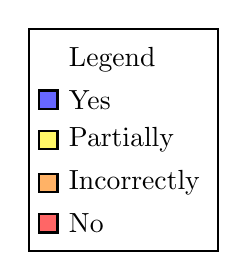
\begin{tikzpicture}
            \matrix [thick, draw=black] {
            \node[label=right:{Legend}] {}; \\
            \node[thick, shape=rectangle, draw=black, fill=blue!60,   label=right:{Yes}        ](0) {}; \\
            \node[thick, shape=rectangle, draw=black, fill=yellow!60, label=right:{Partially}  ](1) {}; \\
            \node[thick, shape=rectangle, draw=black, fill=orange!60, label=right:{Incorrectly}](2) {}; \\
            \node[thick, shape=rectangle, draw=black, fill=red!60,    label=right:{No}         ](3) {}; \\
            };
        \end{tikzpicture}
    \end{subfigure}
    \caption{Breakdown of how many suggestions we made on the \acs{swebok} V4
        \citep{SWEBOK2024} were incorporated into the final version
        \citeyearpar{SWEBOK2025}.}\label{fig:swebokUpdates}
\end{figure*}

\fi

\subsubsection{\textSources{1}}\label{texts}
% Colored \textcolor{Maroon}{maroon}

We consider textbooks to be more credible than papers (see \Cref{papers})
because they are widely used as resources for teaching software engineering and
industry frequently uses them as guides. Although textbooks have smaller sets of
authors, they follow a formal review process before publication. Textbooks used
at McMaster University \citep{Patton2006,PetersAndPedrycz2000,vanVliet2000}
served as the original (albeit ad hoc and arbitrary) starting point of this
research, and we investigate other books as they arise. \addTextEx{}

\subsubsection{\paperSources{1}}\label{papers}
% Colored black

The remaining documents all have much smaller sets of authors and are much less
widespread than those in higher source tiers. While most of these are journal
articles and conference papers, we also include the following document types.
Some of these are not peer-reviewed works but are still useful for
observing how terms are used in practice\thesisissueref{89}:

\begin{itemize}
    \item Report \citep{Kam2008,Gerrard2000a,Gerrard2000b}
    \item Thesis \citep{Bas2024}
          % \item A less-formal classification \citep{KuļešovsEtAl2013}
    \item Website \citep{LambdaTest2024,Pandey2023}
    \item Booklet \citep{SPICE2022}
    \item \ifnotpaper \else ChatGPT \fi \citet{ChatGPT2024} with its claims
          supported by \citet{RusEtAl2008}\ifnotpaper%
              \footnote{\citet[p.~88]{Patton2006} says that if a specific
                  defect is found, it is wise to look for other defects in the
                  same location and for similar defects in other locations, but
                  does not provide a name for this approach. After researching
                  in vain, we ask \citet{ChatGPT2024} to name this test approach
                  but do \emph{not} take its output to be true at face value.
                  \citet{RusEtAl2008} support calling this approach ``defect-based
                  testing'' based on the principle of ``defect clustering''.
                  %   For more information on how and why we use ChatGPT, see
                  %   \Cref{use-of-chatgpt}.
              }\fi
\end{itemize}
